\section{Deux 4-transpositions}

\paragraph{}
If there are two 4-transpositions, there are 12 edges but the minimum number to link 11 points is 10. There are two "joker" edges. Thus

\begin{theorem}
  Si un sggi de degré $4$ sur $A_{11}$ possède exactement deux 4-transposition, alors celles-ci sont sur les positions $\rho_1$ et $\rho_2$.
\end{theorem}

\begin{proof}
  Supposons qu'il existe une 4-transposition en $\rho_0$. Alors celle-ci doit commuter avec $\rho_2$ et $\rho_3$. Ces deux dernières involutions ont au moins deux arêtes chacunes.



  \paragraph{}
  Nous allons utiliser un raisonnement similaire à celui utilisé pour le rang 5. Néanmoins, une différence avec le rang 5 est que les deux involutions que nous ajoutons ($\rho_2$ et $\rho_3$) ne doivent pas commuter entre elles. Dès lors, il est possible, lors de la construction de $\rho_3$, de relier deux points fixés par $\rho_0$ mais pas fixés par $\rho_2$ sans que cela ne pose un problème. Les deux possibilités sont donc les suivantes.

  \begin{enumerate}
    \item Doubler une arête et relier deux points fixés par $\rho_0$.
    \item Former un carré alterné.
  \end{enumerate}

  \paragraph{}
  Le problème se pose quand on choisit ce que doit faire l'involution $\rho_3$. Elle ne peut pas former d'arête double avec $\rho_0$ car il est impossible de les relier après. De même, elle ne peut pas former de carré alterné avec $\rho_0$ car le problème serait le même. Il faut donc utiliser l'involution $\rho_2$ pour résoudre ce problème.

  \paragraph{}
  Pour relier l'arête double, la seule solution est de créer un carré qui contiendra cette arête mais alors ce carré possèderait une arête triple et donc on utiliserait trois arête disponibles alors que nous n'en possèdont que deux. Pour relier le carré alterné, nous pouvons coller un autre carré alterné à celui-ci. On obtient alors le graphe suivant:

  \begin{figure}[H]
    \begin{center}
      \begin{tikzpicture}

        \begin{scope}[every node/.style={circle,draw}]
          \node (1)  at (0,2)  {};
          \node (2)  at (0,0)  {};
          \node (3)  at (2,2)  {};
          \node (4)  at (2,0)  {};
          \node (5)  at (4,2)  {};
          \node (6)  at (4,0)  {};
          \node (7)  at (6,2)  {};
          \node (8)  at (6,0)  {};
          \node (9)  at (8,2)  {};
          \node (10) at (8,0)  {};
          \node (11) at (10,2) {};
        \end{scope}

        \begin{scope}[every node/.style={fill=white}]

          \begin{scope}[every edge/.style={draw}]
            \path (1)  edge node {$0$} (2);
            \path (3)  edge node {$0$} (4);
            \path (5)  edge node {$0$} (6);
            \path (7)  edge node {$0$} (8);
            \path (3)  edge node {$2$} (5);
            \path (4)  edge node {$2$} (6);
            \path (1)  edge node {$3$} (3);
            \path (2)  edge node {$3$} (4);
          \end{scope}
        \end{scope}

      \end{tikzpicture}
      \caption{}
    \end{center}
  \end{figure}

  \paragraph{}
  Maintenant la seule possibilité pour relier les carrés au reste est d'utiliser des arêtes de $\rho_1$. Nous allons donc devoir utiliser deux arêtes de $\rho_1$. Pour relier les points manquants nous avons alors un ou deux points que nous pouvons relier et celui-ci (ceux-ci) sont uniquement reliés par des arêtes de $\rho_1$. La seule possibilité est d'utiliser une arête de $\rho_2$ pour les relier. Donc $\rho_2$ est une 4-transposition. Étudions les deux cas un peu plus en détails.

  \paragraph{}
  Nous ne pouvons utiliser qu'une arête $\rho_2$. En effet dans le cas où nous n'avons qu'une arête $\rho_1$ où nous pouvons attacher qu'une seule arête $\rho_2$ car nous n'avons qu'un point disponible. Dans le cas où nous avons deux points connecté par $\rho_1$, ces deux point faisaient partie des trois points fixes du graphe ci-dessus. Il n'en reste plus qu'un, donc soit nous relions les deux points ensemble soit nous relier le dernier point fixe. Si nous relions les points ensemble, nous ne pouvons plus rien faire.

  \paragraph{}
  Maintenant, nous devons relier le dernier point que nous avons créé, qui est déjà relié par $\rho_2$. Mais nous ne pouvons plus utiliser $\rho_2$. Donc $\rho_2$ est une 3-transposition, ce qui est impossible.

\end{proof}

\begin{theorem}
  All sggi of rank 4 with two 4-transpoisiton on $A_{11}$ are those presented in appendix~\ref{rank4-4-4transpositions} (p.~\pageref{rank4-4-4transpositions})).
\end{theorem}

There are a lot of graph, it is important to be structured. The following classification will be used.

\begin{enumerate}
  \item Choose which structures consume the "joker" edges: two double edges, one double edge and one alternating square or two alternating squares.
  \item Choose the length of the chain between between the two structures.
  \item Choose the distance between one structure and the end of the graph.
\end{enumerate}

\paragraph{}
Once this decision tree is made, finding the graphs is very easy. The structure of appendix~\ref{rank4-4-4transpositions} matches the decision tree. It's important to check that the dual of the current graph has not already be found.

\paragraph{}
This proof is very easy and quite long. If the reader is interested, he can easyly do it.

\begin{theorem}
  None of the sggi presented in appendix~\ref{rank4-4-4transpositions} are C-groups.
\end{theorem}

\begin{proof}
  The analysis will be splitted by the structure used to consume "joker" edges.

  \subsection{Two double edges}

  The following table contains the list of all sggis and some of their subgroup.


\begin{table}[H]
  \centering
  \begin{tabular}{|c|c|c|c|c|c|c|}
    \hline
    Figure & $\Gamma_3$ & $\Gamma_0$ & $\Gamma_{0,3}$ & $\#\Gamma_{0,3}$ & $\Gamma_3 \cap \Gamma_0$ & $\#(\Gamma_3 \cap \Gamma_0)$ \\ \hline

    \ref{r4-1-1} & $A_8 : S_3$ & $A_8 : S_3$ & $D_{30}$ & 30 & $\ge S_5$ & $\ge 120$ \\ \hline
    \ref{r4-1-2} & $A_5 \times 5 : 2$ & $A_8 : S_3$ & $D_{30}$ & 30 &  \\ \hline
    \ref{r4-1-3} & $A_7 \times 2 \times 2 : S_3$ & $A_7 \times 2 \times 2 : S_3$ & $D_{24}$ & 24 &  \\ \hline
    \ref{r4-1-4} & $S_7 \times 2 : 2$ & $A_7  \times 2 \cdot 2 : 2$ & $D_{24}$ & 24 &  \\ \hline
    \ref{r4-1-5} & $A_8 : S_3$ & $A_5 \times 5 : 2$ & $D_{30}$ & 30 &  \\ \hline
    \ref{r4-1-6} & $A_8 : S_3$ & $A_{10}$ & $D_{42}$ & 42 &  \\ \hline
    \ref{r4-1-7} & $A_5 \times 5 : 2$ & $A_{10}$ & $D_{10}$ & 10 &  \\ \hline
    \ref{r4-1-8} & $A_{10}$ & $A_{10}$ & $D_{18}$ & 18 &  \\ \hline
    \ref{r4-1-9} & $A_{10}$ & $A_5 \times 5 : 2$ & $D_{10}$ & 10 &  \\ \hline
    \ref{r4-1-10}& $S_7 \times 2:2$ & $S_9$ & $D_{40}$ & 40 &  \\ \hline
    \ref{r4-1-11}& $A_{10}$ & $A_5 : S_6$ & $D_{10}$ & 10 &  \\ \hline
    \ref{r4-1-12}& $S_9$ & $A_7 \times 2 \times 2:S_3$ & $D_{40}$ & 40 &  \\ \hline
    \ref{r4-1-13}& $A_8 : S_3$ & $A_8 : S_3$ & $D_{30}$ & 30 & \\ \hline
    \ref{r4-1-14}& $A_8 : S_3$ & $A_{10}$ & $D_{42}$ & 42 & \\ \hline
    \ref{r4-1-15}& $A_{10}$ & $A_{10}$ & $D_{18}$ & 18 & \\ \hline
    \ref{r4-1-16}& $S_9$ & $S_9$ & $D_{28}$ & 28 & \\ \hline
    \ref{r4-1-17}& $A_{10}$ & $A_8 : S_3$ & $D_{42}$ & 42 & \\ \hline
    \ref{r4-1-18}& $A_{10}$ & $A_{10}$ & $D_{18}$ & 18 & \\ \hline
    \ref{r4-1-19}& $A_{10}$ & $A_7 \times 2 \times 2 : S_3$ & $D_{42}$ & 42 & \\ \hline
    \ref{r4-1-20}& $S_9$ & $A_5 : S_6$ & $D_{12}$ & 12 & \\ \hline
    \ref{r4-1-21}& $A_7 \times 2 \times 2 : S_{3}$ & $A_{10}$ & $D_{42}$ & 42 & \\ \hline

  \end{tabular}
  \caption{}
\end{table}

  Nous allons donc construire toutes les possibilités et puis prouver, de manière générale, qu'aucun de ces sggi n'est un C-group.

  \paragraph{}
  Remarquons que nous ne pouvons pas former de carré alterné. En effet, les seuls carrés alternés connectable sont de la forme $[\rho_0, \rho_2]$ ou $[\rho_1, \rho_3]$. Mais dans chacun des deux cas, ils utilisent toute les arêtes d'une des deux transpoisition. Les arêtes à placer ne sont donc plus d'un seul bloc et c'est donc impossible.

  \paragraph{}
  Considérons maintenant la 4-transposition $\rho_0$ et la 2-transposition $\rho_2$. Celles-ci doivent partager au moins une arête. Vu l'absence de carré alterné, il y a une arête double entre $\rho_0$ et $\rho_2$. Par dualité, nous trouvons une autre arête double entre $\rho_1$ et $\rho_3$.

  \paragraph{}
  Nous avons donc utilisé toutes nos arêtes en surplus et le reste du graphe doit donc être linéaire. Les arêtes doubles, doiventre être connectées par au moins un des deux côtés. Nous pouvons donc ajouter une arête, respectivement $\rho_1$ et $\rho_2$.

  \paragraph{}
  Il nous reste une arête $\rho_0$ et une arête $\rho_3$, celles-ci doivent être entièrement entourées par des arêtes $\rho_1$ et $\rho_2$. Elle peuvent n'utiliser qu'une arête si elles sont à une extrémité de la chaîne.

  \paragraph{}
  Pour connecter les deux arêtes doubles, nous pouvons utiliser un chaîne de longueur 2, 4, 6 ou 8. Une chaîne de 8 est impossible car alors les deux arêtes doubles seraient aux extrémités, donc les arêtes $\rho_0$ et $\rho_3$ doivent être entièrement entourées. Si l'arête de $\rho_1$ connectant l'arête double n'est pas utilisé pour connecter $\rho_0$, alors toutes les arêtes $\rho_1$ auront été utilisées. Si c'est la même chôse pour $\rho_3$, on a utilisé toutes nos arêtes, il suffit donc de mettre les morceaux ensemble, on a donc le graphe suivant:

  \begin{figure}[H]
    \begin{center}
      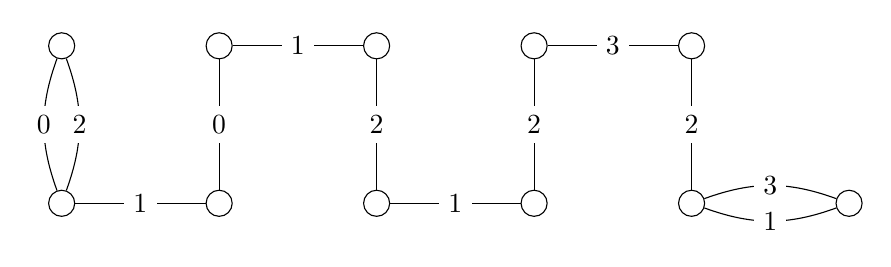
\begin{tikzpicture}

        \begin{scope}[every node/.style={circle,draw}]
          \node (1)  at (0,2)  {};
          \node (2)  at (0,0)  {};
          \node (3)  at (2,0)  {};
          \node (4)  at (2,2)  {};
          \node (5)  at (4,2)  {};
          \node (6)  at (4,0)  {};
          \node (7)  at (6,0)  {};
          \node (8)  at (6,2)  {};
          \node (9)  at (8,2)  {};
          \node (10) at (8,0)  {};
          \node (11) at (10,0) {};
        \end{scope}

        \begin{scope}[every node/.style={fill=white}]

          \begin{scope}[every edge/.style={draw}]
            \path (1)  edge[bend right=20] node {$0$} (2);
            \path (3)  edge node {$0$} (4);
            \path (2)  edge node {$1$} (3);
            \path (4)  edge node {$1$} (5);
            \path (6)  edge node {$1$} (7);
            \path (10) edge[bend right=20] node {$1$} (11);
            \path (1)  edge[bend left=20] node {$2$} (2);
            \path (5)  edge node {$2$} (6);
            \path (7)  edge node {$2$} (8);
            \path (9)  edge node {$2$} (10);
            \path (8)  edge node {$3$} (9);
            \path (10) edge[bend left=20] node {$3$} (11);
          \end{scope}
        \end{scope}

      \end{tikzpicture}
      \caption{[1, 1075, 5720, 153]}
    \end{center}
  \end{figure}

  \paragraph{}
  Dans le cas contraire, au moins un arête pour connecter une arête double est aussi utilisée pour connecter une arête extémale. Suppososon que celà soit $\rho_1$. Le graphe est actuellement le suivant:

  \begin{figure}[H]
    \begin{center}
      \begin{tikzpicture}

        \begin{scope}[every node/.style={circle,draw}]
          \node (1)  at (0,2)  {};
          \node (2)  at (0,0)  {};
          \node (3)  at (2,0)  {};
          \node (4)  at (2,2)  {};
          \node (5)  at (4,2)  {};
          \node (6)  at (4,0)  {};
          \node (7)  at (6,0)  {};
          \node (8)  at (6,2)  {};
          \node (9)  at (8,2)  {};
          \node (10) at (8,0)  {};
          \node (11) at (10,0) {};
        \end{scope}

        \begin{scope}[every node/.style={fill=white}]

          \begin{scope}[every edge/.style={draw}]
            \path (1)  edge[bend right=20] node {$0$} (2);
            \path (3)  edge node {$0$} (4);
            \path (2)  edge node {$1$} (3);
            \path (4)  edge node {$1$} (5);
            %\path (4)  edge node {$1$} (5);
            \path (10) edge[bend right=20] node {$1$} (11);
            \path (1)  edge[bend left=20] node {$2$} (2);
            %\path (6)  edge node {$2$} (11);
            %\path (7)  edge node {$2$} (10);
            \path (9)  edge node {$2$} (10);
            %\path (9)  edge node {$3$} (10);
            \path (10) edge[bend left=20] node {$3$} (11);
          \end{scope}
        \end{scope}

      \end{tikzpicture}
      \caption{[1, 1075, 5720, 153]}
    \end{center}
  \end{figure}

  \paragraph{}
  Au delà de l'arête $\rho_1$, ce graphe ne peut être complété que d'une seule manière:

  \begin{figure}[H]
    \begin{center}
      \begin{tikzpicture}

        \begin{scope}[every node/.style={circle,draw}]
          \node (1)  at (0,2)  {};
          \node (2)  at (0,0)  {};
          \node (3)  at (2,0)  {};
          \node (4)  at (2,2)  {};
          \node (5)  at (4,2)  {};
          \node (6)  at (4,0)  {};
          \node (7)  at (6,0)  {};
          \node (8)  at (6,2)  {};
          \node (9)  at (8,2)  {};
          \node (10) at (8,0)  {};
          \node (11) at (10,0) {};
        \end{scope}

        \begin{scope}[every node/.style={fill=white}]

          \begin{scope}[every edge/.style={draw}]
            \path (1)  edge[bend right=20] node {$0$} (2);
            \path (3)  edge node {$0$} (4);
            \path (2)  edge node {$1$} (3);
            \path (4)  edge node {$1$} (5);
            %\path (4)  edge node {$1$} (5);
            \path (10) edge[bend right=20] node {$1$} (11);
            \path (1)  edge[bend left=20] node {$2$} (2);
            \path (5)  edge node {$2$} (6);
            %\path (7)  edge node {$2$} (10);
            \path (9)  edge node {$2$} (10);
            %\path (9)  edge node {$3$} (10);
            \path (10) edge[bend left=20] node {$3$} (11);
          \end{scope}
        \end{scope}

      \end{tikzpicture}
      \caption{[1, 1075, 5720, 153]}
    \end{center}
  \end{figure}

  \paragraph{}
  Maintenant, nous avons 2 possibilités, une chaîne $\rho_1, \rho_2, \rho_3$ ou $\rho_3, \rho_2, \rho_1$, ce qui nous donne les deux graphes suivants:

  \begin{figure}[H]
    \begin{center}
      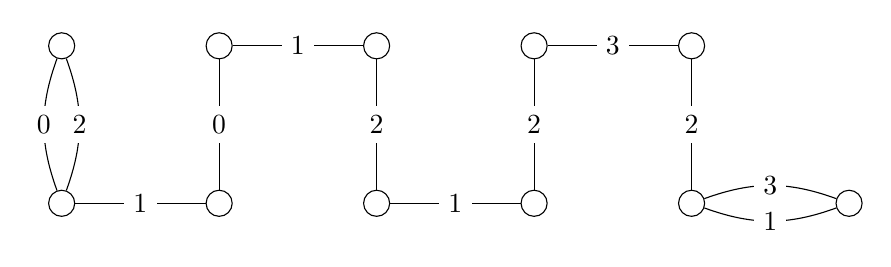
\begin{tikzpicture}

        \begin{scope}[every node/.style={circle,draw}]
          \node (1)  at (0,2)  {};
          \node (2)  at (0,0)  {};
          \node (3)  at (2,0)  {};
          \node (4)  at (2,2)  {};
          \node (5)  at (4,2)  {};
          \node (6)  at (4,0)  {};
          \node (7)  at (6,0)  {};
          \node (8)  at (6,2)  {};
          \node (9)  at (8,2)  {};
          \node (10) at (8,0)  {};
          \node (11) at (10,0) {};
        \end{scope}

        \begin{scope}[every node/.style={fill=white}]

          \begin{scope}[every edge/.style={draw}]
            \path (1)  edge[bend right=20] node {$0$} (2);
            \path (3)  edge node {$0$} (4);
            \path (2)  edge node {$1$} (3);
            \path (4)  edge node {$1$} (5);
            \path (6)  edge node {$1$} (7);
            \path (10) edge[bend right=20] node {$1$} (11);
            \path (1)  edge[bend left=20] node {$2$} (2);
            \path (5)  edge node {$2$} (6);
            \path (7)  edge node {$2$} (8);
            \path (9)  edge node {$2$} (10);
            \path (8)  edge node {$3$} (9);
            \path (10) edge[bend left=20] node {$3$} (11);
          \end{scope}
        \end{scope}

      \end{tikzpicture}
      \caption{[1, 1075, 5720, 153]}
    \end{center}
  \end{figure}

  \begin{figure}[H]
    \begin{center}
      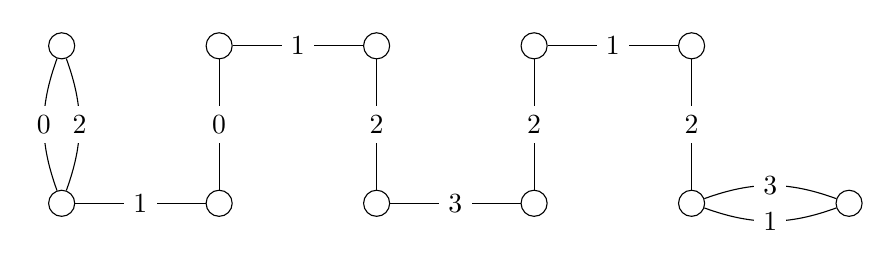
\begin{tikzpicture}

        \begin{scope}[every node/.style={circle,draw}]
          \node (1)  at (0,2)  {};
          \node (2)  at (0,0)  {};
          \node (3)  at (2,0)  {};
          \node (4)  at (2,2)  {};
          \node (5)  at (4,2)  {};
          \node (6)  at (4,0)  {};
          \node (7)  at (6,0)  {};
          \node (8)  at (6,2)  {};
          \node (9)  at (8,2)  {};
          \node (10) at (8,0)  {};
          \node (11) at (10,0) {};
        \end{scope}

        \begin{scope}[every node/.style={fill=white}]

          \begin{scope}[every edge/.style={draw}]
            \path (1)  edge[bend right=20] node {$0$} (2);
            \path (3)  edge node {$0$} (4);
            \path (2)  edge node {$1$} (3);
            \path (4)  edge node {$1$} (5);
            \path (8)  edge node {$1$} (9);
            \path (10) edge[bend right=20] node {$1$} (11);
            \path (1)  edge[bend left=20] node {$2$} (2);
            \path (5)  edge node {$2$} (6);
            \path (7)  edge node {$2$} (8);
            \path (9)  edge node {$2$} (10);
            \path (6)  edge node {$3$} (7);
            \path (10) edge[bend left=20] node {$3$} (11);
          \end{scope}
        \end{scope}

      \end{tikzpicture}
      \caption{[1, 1075, 5720, 153]}
    \end{center}
  \end{figure}

  \paragraph{}
  Il nous faut encore prouver qu'aucun de ces trois cas n'est un C-group.

\subsection{One double edge and one alternating square}

\subsection{Two alternating squares}
  \paragraph{}
  This section can be done very easily by doing the same procedure that for the previous one.

  \begin{table}[H]
    \centering
    \begin{tabular}{|c|c|c|c|c|c|c|}
      \hline
      Figure & $\Gamma_3$ & $\Gamma_0$ & $\Gamma_{0,3}$ & $\#\Gamma_{0,3}$ & $\Gamma_3 \cap \Gamma_0$ & $\#(\Gamma_3 \cap \Gamma_0)$ \\ \hline

      \ref{r4-3-1} & $S_9$ & $S_9$ & $D_{28}$ & 28 & $\ge S_7$ & $\ge 5040$ \\ \hline
      \ref{r4-3-2} & $S_9$ & $A_8 : S_3$ & $D_{30}$ & 30 & $\ge S_8$ & $\ge 5040$  \\ \hline
      \ref{r4-3-3} & $S_9$ & $S_9$ & $D_{28}$ & 28 & $\ge S_7$ & $\ge 5040$ \\ \hline
      \ref{r4-3-4} & $A_8 : S_3$ & $A_8 : S_3$ & $D_{30}$ & 30 & $\ge S_5$ & $\ge 120$ \\ \hline
      \ref{r4-3-5} & $A_8 : S_3$ & $A_8 : S_3$ & $D_{30}$ & 30 & $\ge S_5$ & $\ge 120$ \\ \hline
      \ref{r4-3-6} & $A_8 : S_3$ & $S_9$ & $D_{12}$ & 12 & $\ge S_6$ & $\ge 720$ \\ \hline
      \ref{r4-3-7} & $A_8 : S_3$ & $A_8 : S_3$ & $D_{30}$ & 30 & $\ge S_5$ & $\ge 120$  \\ \hline
      \ref{r4-3-8} & $S_7 \times D_8$ & $S_9$ & $D_{40}$ & 40 & $\ge S_7$ & $\ge 5040$ \\ \hline
      \ref{r4-3-9} & $S_7 \times D_8$ & $S_9$ & $D_{40}$ & 40 & $\ge S_7$ & $\ge 5040$ \\ \hline
      \ref{r4-3-10}& $S_9$ & $S_9$ & $D_{28}$ & 40 & $\ge S_9$ & $\ge 5040$ \\ \hline

    \end{tabular}
  \end{table}

\end{proof}
